\section{Obiettivi} 
\label{obiettivi}
Come accennato nella sezione \ref{intro}, l'obiettivo di questo elaborato è stato realizzare un applicativo da riga di comando per piattaforme UNIX scritto interamente in Python, in grado di estrarre la bibliografia da un articolo scientifico caratterizzato delle seguenti proprietà: in lingua inglese, in formato PDF e in cui l'informazione sia codificata sotto forma di testo, escludendo quindi l'analisi su PDF creati come immagini.\\ 
Lo scopo quindi è quello di localizzare la bibliografia ed effettuato ciò, estrarre le voci bibliografiche, evidenziandone il titolo. A questa prima parte più focalizzata sul \textit{retrieval}, ne è seguita un' altra più pratica: si è voluto correggere gli errori del titolo/entry derivanti dall' estrazione non perfetta, reperire in Rete una pagina di approfondimento dell'articolo e infine scarcarsi sia il BibTex dell'articolo citato sia l'articolo stesso in formato PDF. Infine si è deciso di rendere tutte le informazioni visibili tramite un file HTML di indice. Quindi se da un lato l'applicativo prende come input un insieme di PDF di articoli da analizzare, dall' altro invece produce come output un file HTML contenente la bibliografia estratta in cui a ciascuna voce è essociato un collegamento ipertestuale verso la risorsa Web correlata, se esiste, il BibTex e il collegamento al PDF scaricato.\\
Vista l'abbondanza di opzioni con cui è stato sviluppato l'applicativo, è stata inserita la possibilità di personalizzarne l'esecuzione da linea di comando, impostando i vari parametri che attivano o disattivano le opzioni.\\ Questa prima parte di sviluppo è approfondita nella sezione \ref{software}.
Una volta concluso lo sviluppo, segue il secondo obiettivo dell'elaborato: eseguire dei test su una \textit{suite} di articoli in modo da testarne sia il funzionamento sia la qualità della ricerca in termini di precisione per alcune caratteristiche come la correttezza sulle voci estratte, la correttezza dei titoli evidenziati e la pertinenza della URL trovata online con l'articolo. Tutti i risultati saranno appuntati in delle relative tabelle e commentati.\\
Finita questa parte di analisi dei risultati, reperibile nelle sezione \ref{esperimenti}, si stileranno delle conclusione sul lavoro svolto, sui risultati ottenuti e sugli sviluppi futuri. Nella figura \ref{fig:layout} è riportato il diagramma di alto livello di come si è progettata l'esecuzione di \textit{pdftoref}:

\begin{figure}[b]
\begin{center}
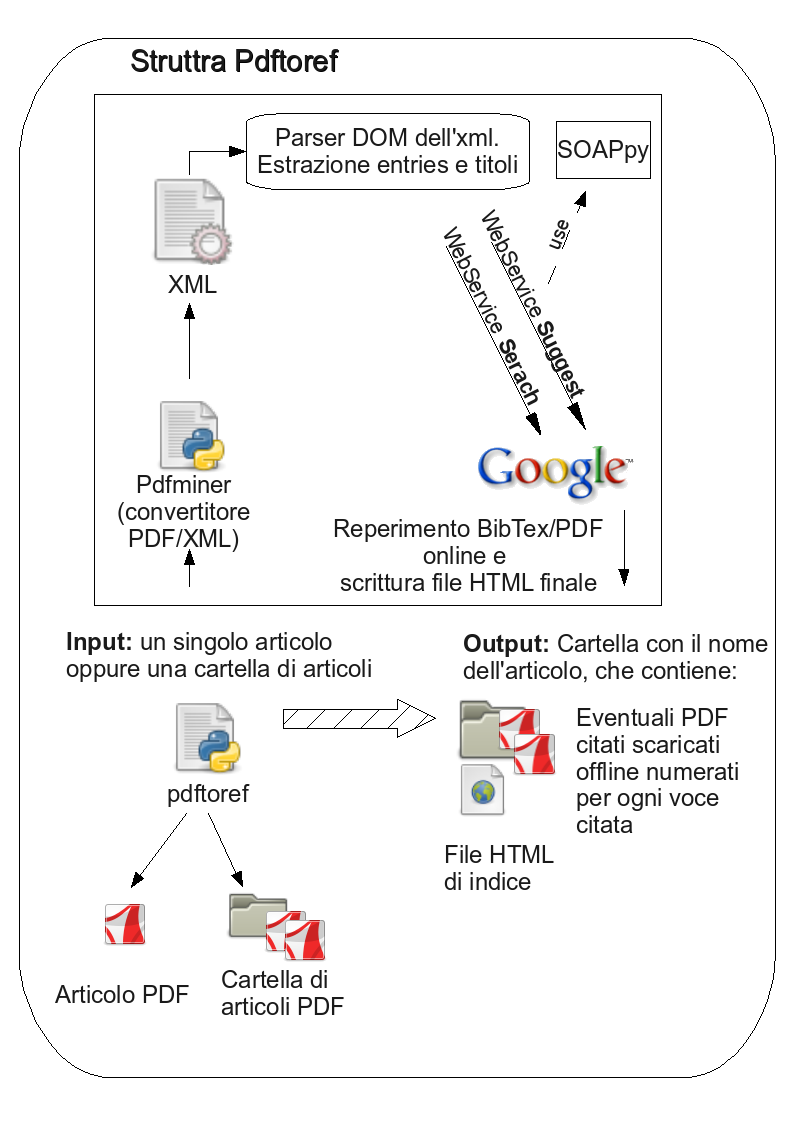
\includegraphics[scale=0.55]{struttura.png}
\end{center}
\caption[Diagramma ad alto livello dei passi eseguiti dall'applicativo]{\textit{Diagramma ad alto livello dei passi eseguiti da pdftoref. Nella figura si nota l'uso del tool PdfMiner per per la conversione in XML. Inoltre si notano le interrogazione al WebService di Google sia per il miglioramento del titolo tramite \textbf{Google Suggest} sia per la ricerca della URL sulle più note scientific digital libraries.}}
\label{fig:layout}
\end{figure}

% quali: la possibilità di passargli un file di input oppure una  directory, la possiblità di attivare la ricerca della URL, l'estrazione de BibTex, e il downloading dei PDF. Si è ritenuto necessario implementare questo poichè al variare dei parametri immessi, varia molto anche il tempo di esecuzione dell'applicativo.
